\documentclass[spanish,10.5pt,twoside,a4paper]{article}
\newcommand{\titulo}{Laboratorio - Fund. de las Comunicaciónes}
\newcommand{\tituloHeader}{\titulo}
\newcommand{\autor}{Christian Yoel Herrera}
\newcommand{\establecimiento}{Facultad de Ingenieria, UNLP}

%----------------------------------------------------------------------------------------
%	PAQUETES GENERALES
%----------------------------------------------------------------------------------------
%----------------------------------------------------------------------------------------
%	PAQUETES GENERALES
%----------------------------------------------------------------------------------------
\usepackage[spanish,es-noshorthands]{babel} % Configuración para palabras en Español
\usepackage{microtype} 						% Proporciona características avanzadas de microtipografía
\usepackage{XCharter} 						% Proporciona una familia de fuentes basada en la fuente Charter
\usepackage{lettrine} 						% Paquete para acentuar la primer letra de un texto (lettrine)
\usepackage{amsmath,amsfonts,amsthm} 		% Paquetes para matemáticas
\usepackage{graphicx} 						% Requerido para agregar imágenes
\usepackage{svg}
\usepackage{float}							% Requerido para el posicionamiento flotante
\usepackage{tcolorbox}						% Permite hacer recuadros para definiciones
\usepackage{multicol}						% Multicolumnas
\usepackage[hidelinks]{hyperref}			% Este paquete se utiliza para manejar enlaces dentro del documento
\usepackage{color}							% Permite colocar colores a los textos
\usepackage{circuitikz}						% Permite crear circuitos eléctricos




%----------------------------------------------------------------------------------------
%	MARGINS AND SPACING
%----------------------------------------------------------------------------------------
\usepackage{geometry}
\geometry{
	top=1cm,
	bottom=1cm,
	left=1cm,
	right=1cm,
	includehead,
	includefoot,
	%showframe, % Descomentar para visualizar los limites
}
\setlength{\columnsep}{5mm} 				% Separacion entre columnas
% \setlength{\columnseprule}{0.1mm} 		% Linea entre columnas
\usepackage{titlesec}						% Permite modificar los espacios de los titulos
\titlespacing{\section}{0pt}{10pt}{5pt}		% Izquierda del titulo, Antes y despues del mismo



%----------------------------------------------------------------------------------------
%	ENCABEZADO Y PIE DE PAGINA
%----------------------------------------------------------------------------------------
\usepackage{fancyhdr}	% Permite modificar los Encabezados y Pie de Pagina
\usepackage{lastpage} 	% Used to determine the number of pages in the document (for "Page X of Total")
\pagestyle{fancy}
\fancyhf{}
\renewcommand{\headrulewidth}{1pt}	% Separacion post-header
\renewcommand{\footrulewidth}{1pt}	% Separacion pre-footer
\fancyfoot[OR, EL]{Pagina \thepage/\pageref*{LastPage}}
\fancyfoot[OL, ER]{\autor}
\fancyhead[OR, EL]{\today}
\fancyhead[OL, ER]{\tituloHeader}


%----------------------------------------------------------------------------------------
%	FORMATO DEL TITULO Y DEL RESUMEN COMO COMANDO
%----------------------------------------------------------------------------------------
\fancypagestyle{firstpage}{ 		% Solo para la pagina que tenga "\thispagestyle{firstpage}"
	\fancyhead{}
	\renewcommand{\headrulewidth}{0pt}
}
\newcommand{\TituloyResumen}[2]{
	\thispagestyle{firstpage}
	\vspace*{-1.5cm}

	% TITULO
	\begin{center}
		{\huge\bfseries \titulo}\vspace{5mm}\break
		{\large \autor}\break
		{\establecimiento}
	\end{center}

	% RESUMEN
	\begin{center}
		\rule{\linewidth}{0.1mm}
		\begin{flushleft}
			\begin{Large}
				\textbf{Resumen}
			\end{Large}\break
			#1
			\vspace{3mm}\break
			\textit{\textbf{Palabras Claves}}: #2
		\end{flushleft}
		\vspace{-\baselineskip}
		\rule{\linewidth}{0.1mm}
	\end{center}

	% FECHA
	\begin{center}
		\textit{\today}
	\end{center}
}



%----------------------------------------------------------------------------------------
%	TEXTO EN GENERAL
%----------------------------------------------------------------------------------------
\usepackage{parskip}							% Al usarlo, elimina todas las sangrias.
\setlength{\parindent}{0pt} 					% Elimina la sangría
\setlength{\parskip}{6pt plus 1pt minus 1pt} 	% Separacion base: 6pt, Maximo adicional 2pt y minimo adicional 1pt
\setlength{\headheight}{13.6pt}



%----------------------------------------------------------------------------------------
%	CONFIGURACION DEL CUERPO (TABLAS Y FIGURAS)
%----------------------------------------------------------------------------------------
\usepackage{booktabs}		% Para centrar las tablas
\definecolor{GrayCaptions}{rgb}{0.5,0.5,0.5}
\usepackage[
	font={footnotesize, color=GrayCaptions},   % Aplica el color a los captions
	figurename=Imagen,    % Cambia el nombre de las figuras a "Imagen"
	tablename=Tabla,      % Cambia el nombre de las tablas a "Tabla"
	labelfont={it}        % Aplica itálico a las etiquetas
]{caption}
\setlength{\abovecaptionskip}{5pt plus 2pt minus 2pt} % Separacion de los 'captions' con el objeto
\setlength{\belowcaptionskip}{-12pt plus 2pt minus 2pt} % Separacion de los 'captions' con el texto que continua.




%----------------------------------------------------------------------------------------
%	BIBLIOGRAFIA (Para deshabilitar, comentar lo siguiente)
%----------------------------------------------------------------------------------------
\usepackage{csquotes}
\usepackage[
backend=biber,
style=apa,
sortcites,
url=true
]{biblatex}
\addbibresource{Bibliografia.bib}







%%%%%%%%%%%%%% CUERPO %%%%%%%%%%%%%%
\begin{document}
	\TituloyResumen{
		En este informe se desarrolla el estudio del procesamiento digital de señales utilizando el Dongle Receptor de SDR y el Software MatLab.
	}{
		ING, UNLP, SDR, FM, MatLab, MPX
	}

	% CUERPO
	\begin{multicols*}{2}	
		\section*{Introducción}
\lettrine[lines=2,findent=4pt,nindent=0pt]{E}{\normalfont n el ámbito de las modulaciones analógicas, se analizaran algunos aspectos sobre la modulación FM, especificamente en estaciones locales utilizando el Dongle USB que incorpora un sintonizador (R820T2) y un demodulador digital (RTL2832U). En primer lugar se analizara el espectro de frecuencias en la banda de FM comercial y finalmente, descargando las muestras se demodulará el audio utilizando el software MatLab.}
\vspace{3mm}
		
		\section*{Primera Vuelta}
\subsection*{Barrido del Espectro FM}
En Argentina, la banda de frecuencias para el servicio de FM se encuentra entre los $88MHz$ y los $108MHz$. Utilizando el analizador de espectro, se realizó un barrido de frecuencias en la banda de FM, y se eligió la frecuencia de \textbf{$103.7MHz$}. 
Se muestra en la siguiente imagen el espectro cuando se posiciona el filtro pasa-banda centrado en la frecuencia de la portadora y con un ancho de banda de $264kHz$.
\begin{figure}[H]
    \centering
    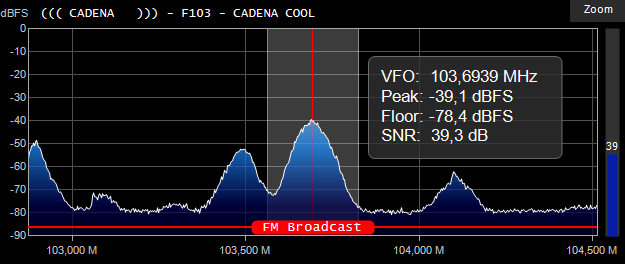
\includegraphics[width=0.9\columnwidth]{images/1.1-rds-103.4MHz.png}
    \caption{Espectro de la frecuencia $103.7MHz$}
    \label{fig:imagen1}
\end{figure}
En esta frecuencia, se pudo observar gracias al plugin \textbf{\textit{FM MPX Spectrum}} que el espectro no es esencialmente el audio en la banda de $0 \sim 15kHz$. Lo que se tiene es la señal \textbf{MPX} que utiliza los dos canales de audio (L y R) para formar el espectro de la imagen \hyperref[fig:imagen2]{Imagen 2}:
\begin{itemize}
	\item El espectro de la suma de los canales.
	\item La frecuencia piloto de $19kHz$.
	\item El espectro de la resta de los canales que posteriormente es modulado en AM para centrarlo en $38kHz$
	\item Y finalmente, el espectro del mensaje RDS que es un mensaje digital que se modula y se agrega al espectro.
\end{itemize}
Dado que el espectro llega mas allá de los $15kHz$, el ancho de banda de Carson ahora será de $264kHz$ ya que si la banda base es de $W=57kHz$, y la máxima desviación de frecuencia se define en $75kHz$, entonces:
$$
BW_{c} = 2\left( \dfrac{75kHz}{57kHz}+ 1 \right) \cdot 57kHz = 264kHz
$$
Por este motivo, se utilizó anteriormente el filtro pasa-banda con un ancho de banda igual a $BW_{c}$.
\begin{figure}[H]
    \centering
    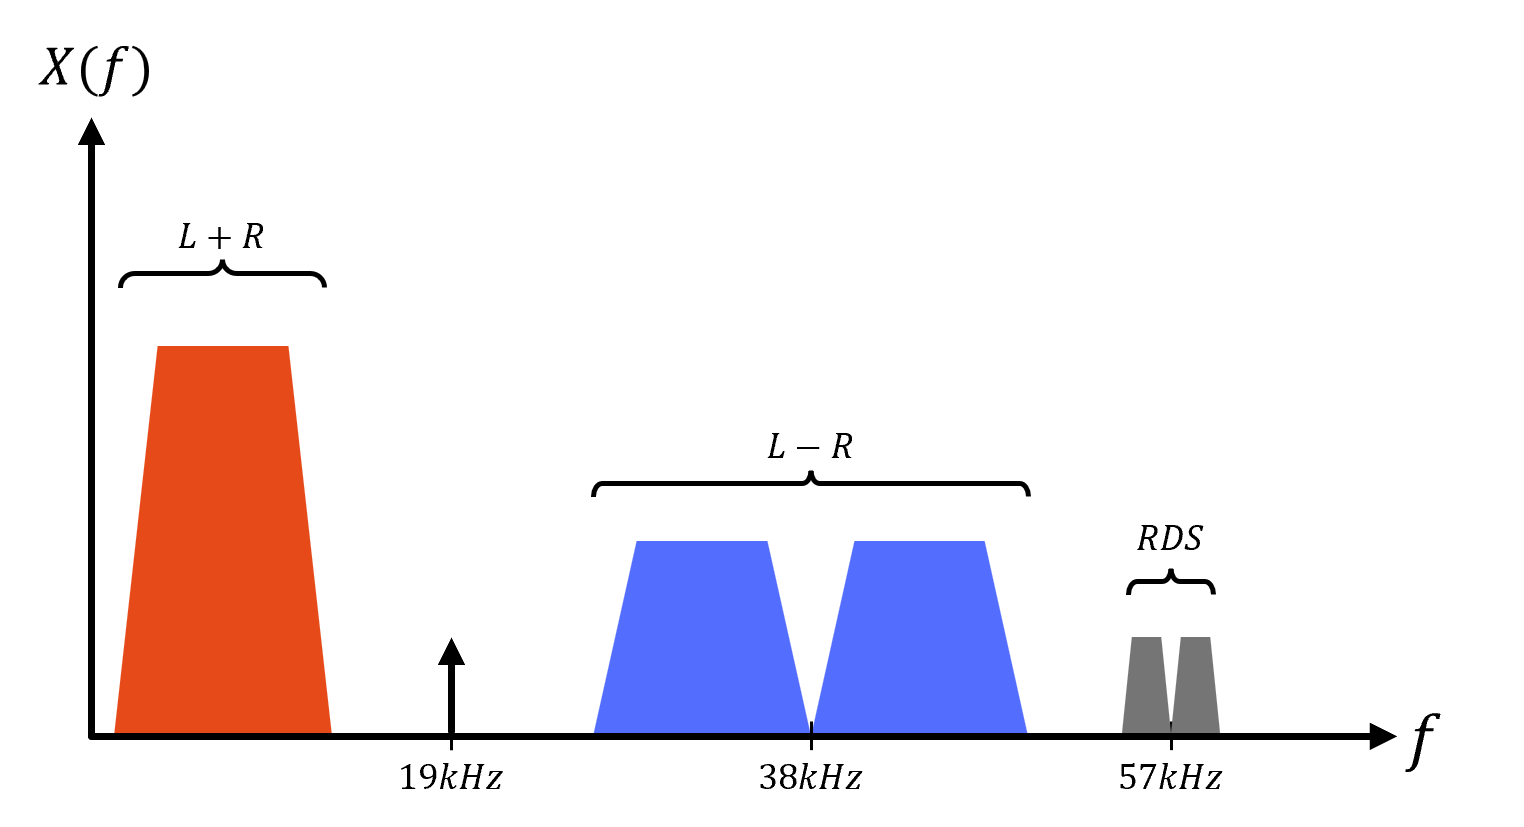
\includegraphics[width=0.8\columnwidth]{images/1.2-espectro-mpx.png}
    \caption{Espectro de una señal MPX}
    \label{fig:imagen2}
\end{figure}

El hecho de ir reduciendo la banda de paso del filtro provoca que se reciba menos potencia de la señal, lo que se traduce en una menor relación señal a ruido, de esta forma se puede observar que la señal de audio se va perdiendo a medida que se reduce el ancho de banda del filtro.

\begin{figure}[H]
    \centering
    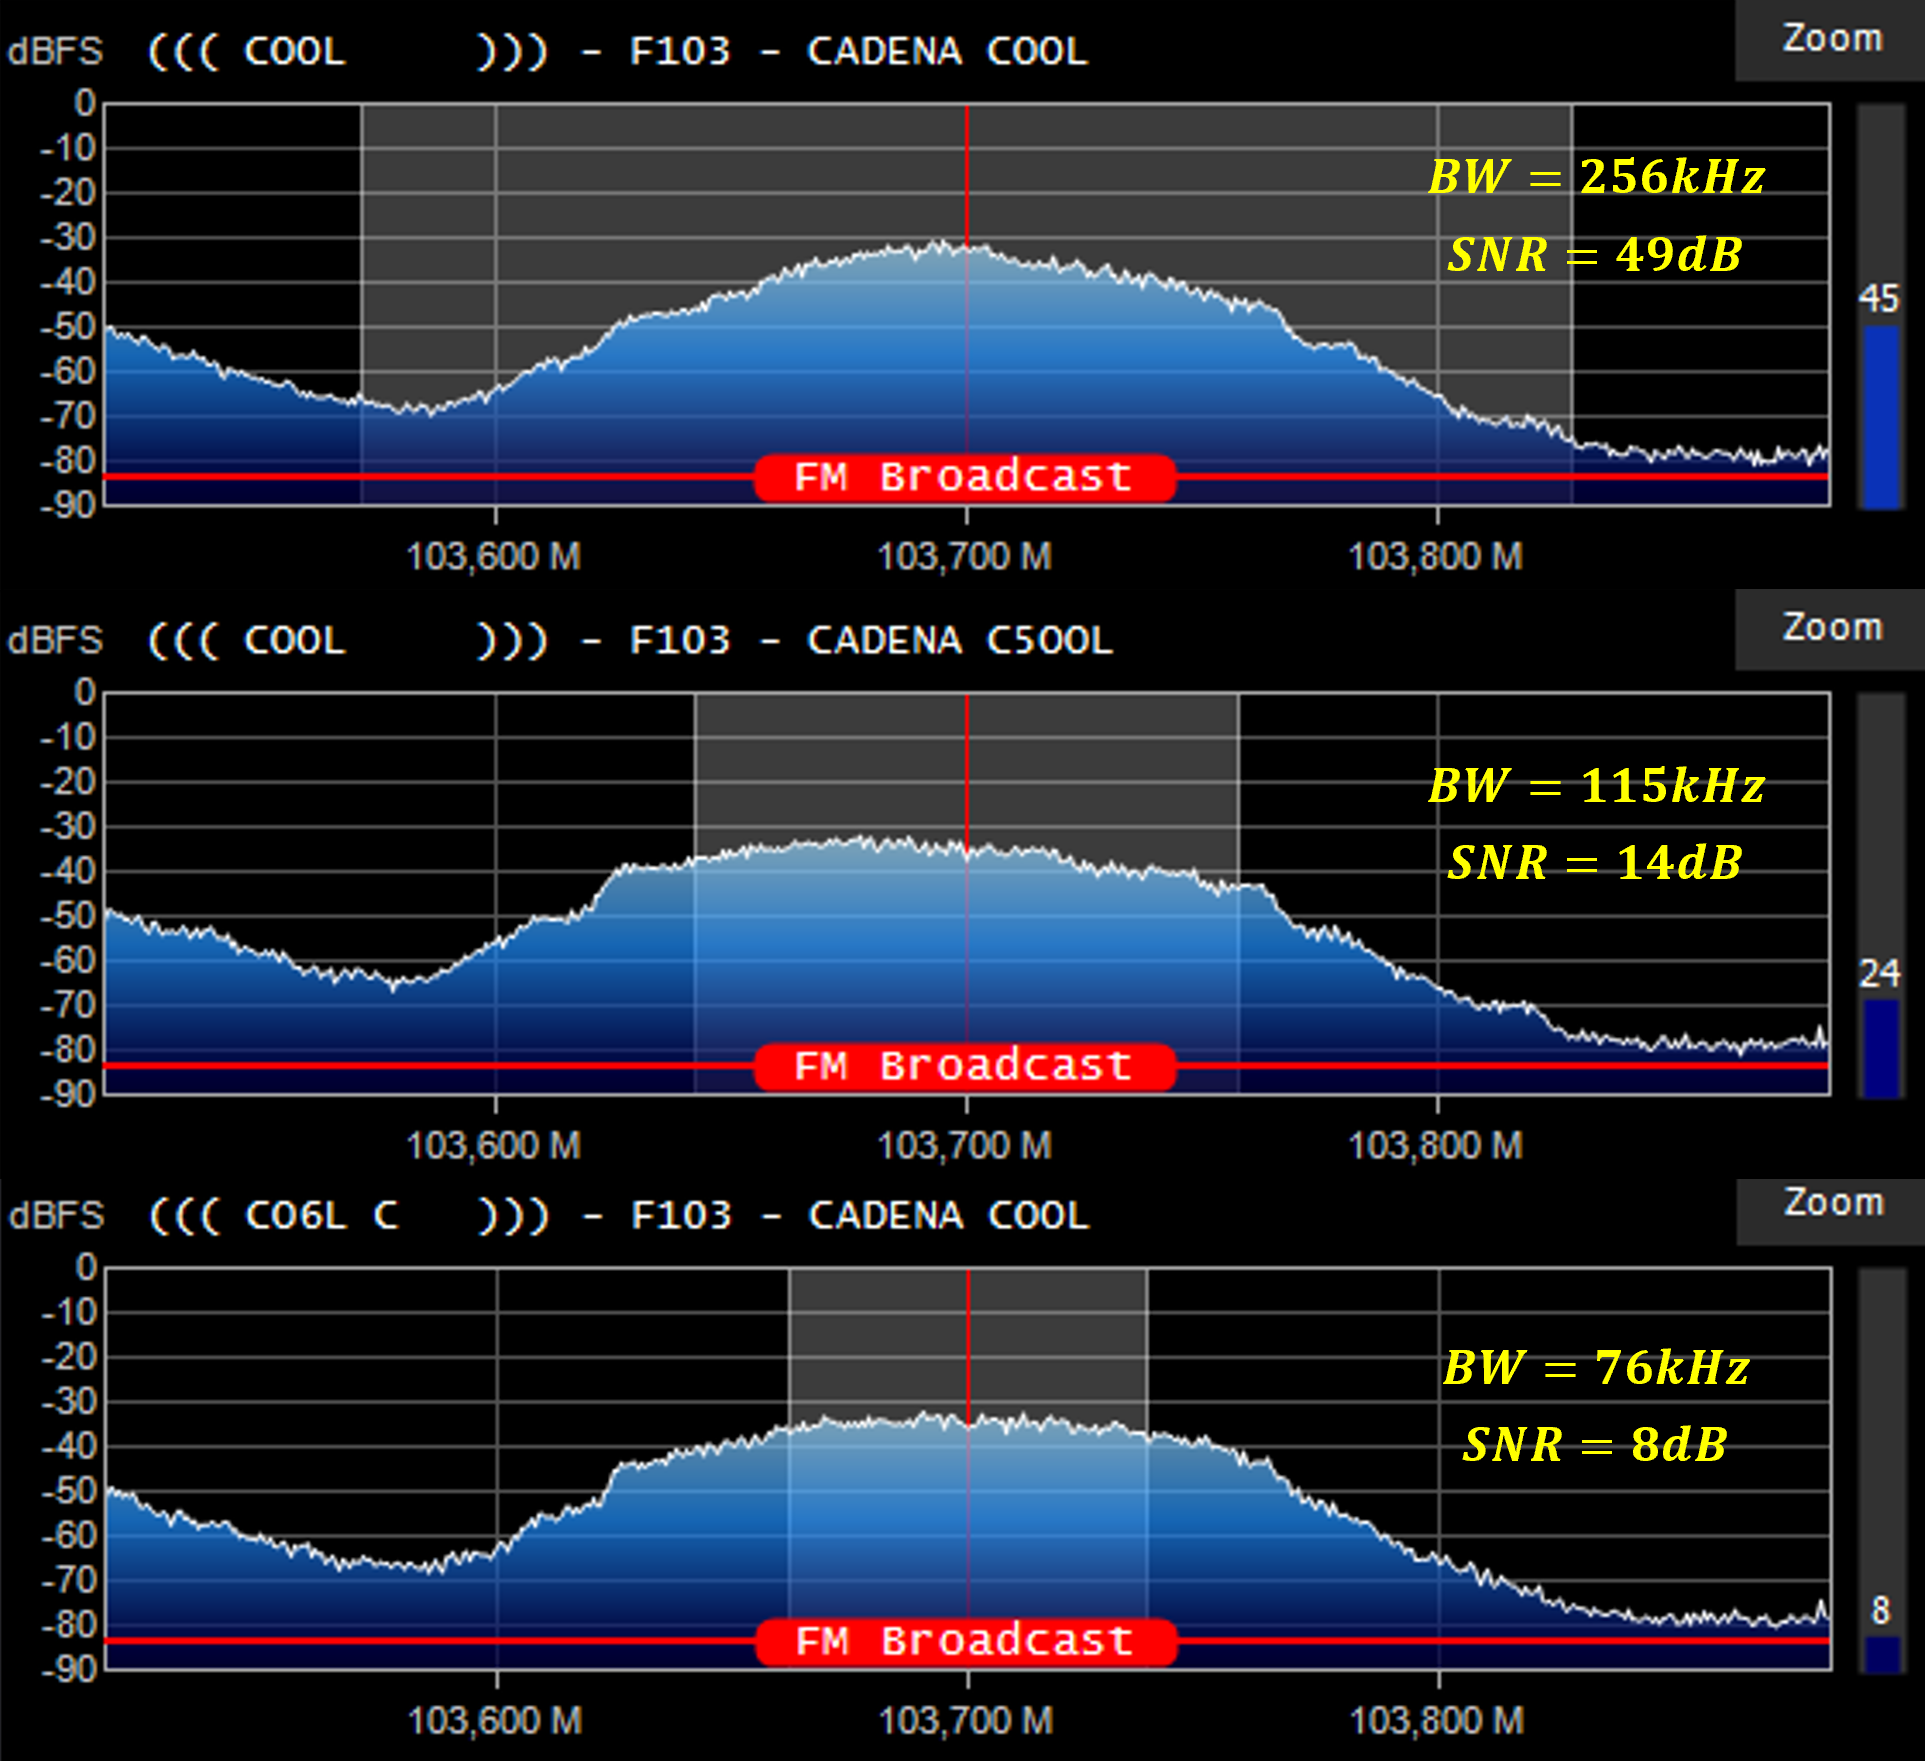
\includegraphics[width=0.9\columnwidth]{images/1.3-mod-bw.png}
    \caption{SNR con distintos anchos de banda}
    \label{fig:imagen3}
\end{figure}

Si la disminución es tal que se pierde parte del espectro de la resta de los canales (L-R en la \hyperref[fig:imagen2]{Imagen 2}), entonces ya no se podrá demodular y escuchar en modo Estéreo.

En el caso de aumentar o disminuir la ganancia del receptor SDR, se puede observar que la señal de audio se distorsiona, y es en parte por aumentar la potencia de ruido, el cual hace que supere en algunos casos la potencia de las estaciones que transmiten.


\hspace{1cm}
		\section*{SDR + MatLab}
\subsection*{Espectro en Análisis}
Utilizando el software MatLab, se realizó el análisis de la señal de radio FM en la frecuencia de $103.7MHz$. Se obtuvo la densidad espectral de potencia, el cual se muestra en la siguiente imagen.
\begin{figure}[H]
    \centering
    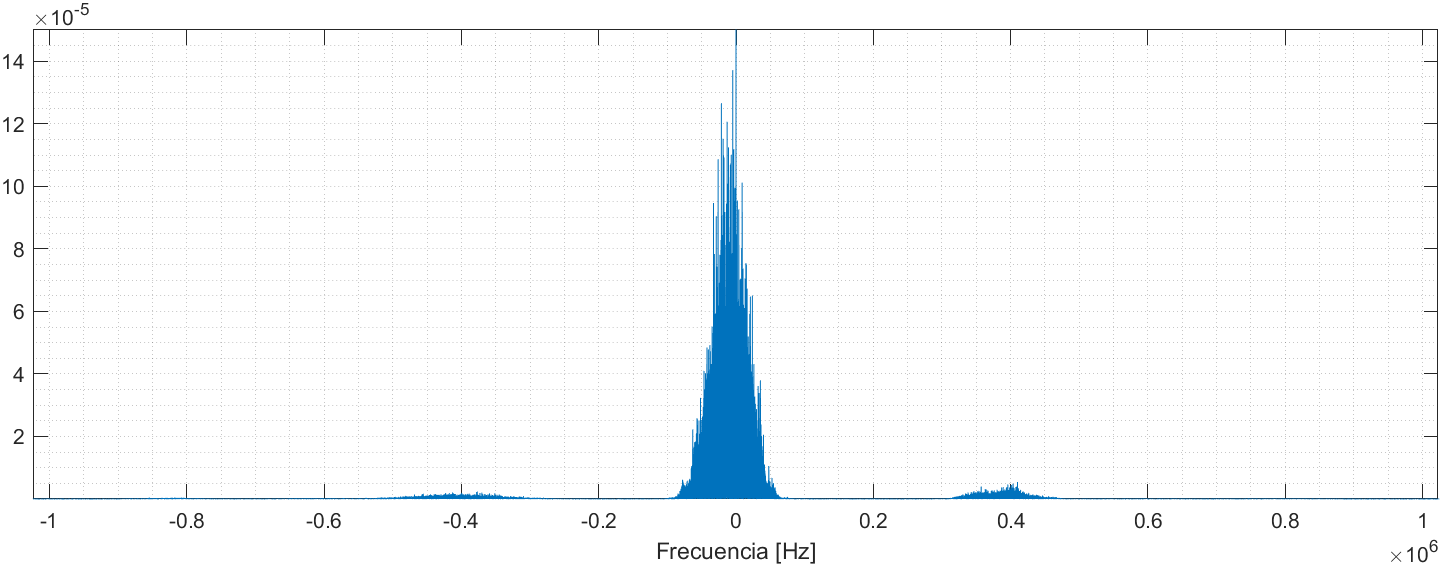
\includegraphics[width=\columnwidth]{images/2.1-original.png}
    \caption{Espectro de la señal de $103.7 MHz$}
    \label{fig:imagen4}
\end{figure}
En tal espectro se ve que existen componentes en la banda de los $264kHz$ pero se también se adiciona un espectro centrado en los $400kHz$ aproximadamente. Esto no corresponde a la estación buscada con lo cual utiliza un filtro butterworth de orden 5.
\begin{figure}[H]
    \centering
    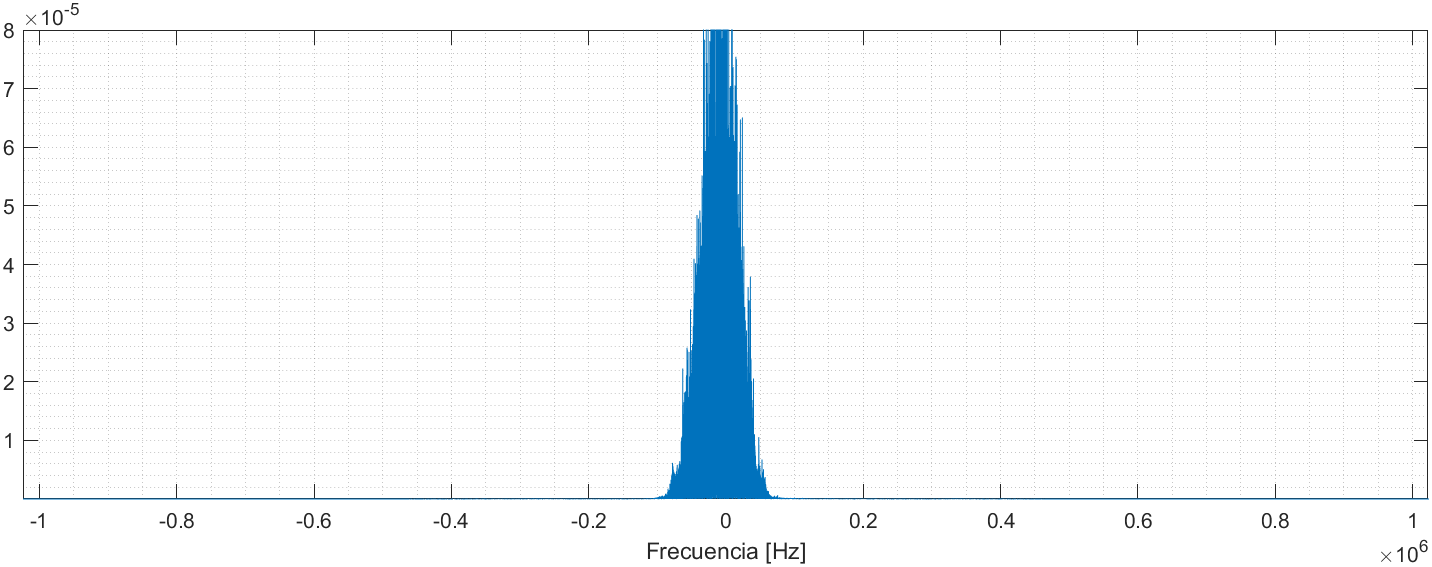
\includegraphics[width=\columnwidth]{images/2.2-filtrando.png}
    \caption{Espectro filtrado}
    \label{fig:imagen5}
\end{figure}
Una vez eliminado el espectro no deseado, se agrega un diezmado para que el procesamiento digital sea mas rápido al reducir la cantidad de muestras a procesar. Si se considera tener una señal que tenga un espectro de muestras entre $-120kHz$ y $120kHz$ cuando la frecuencia de muestreo era de $2048kHz$, se requiere:
$$
N_{1} = \frac{f_s}{2f_{lim}} = \frac{2048kHz}{2 \cdot 120kHz} = 8.53
$$
Utilizando $N_{1}=9$ se obtiene el espectro siguiente:
\begin{figure}[H]
    \centering
    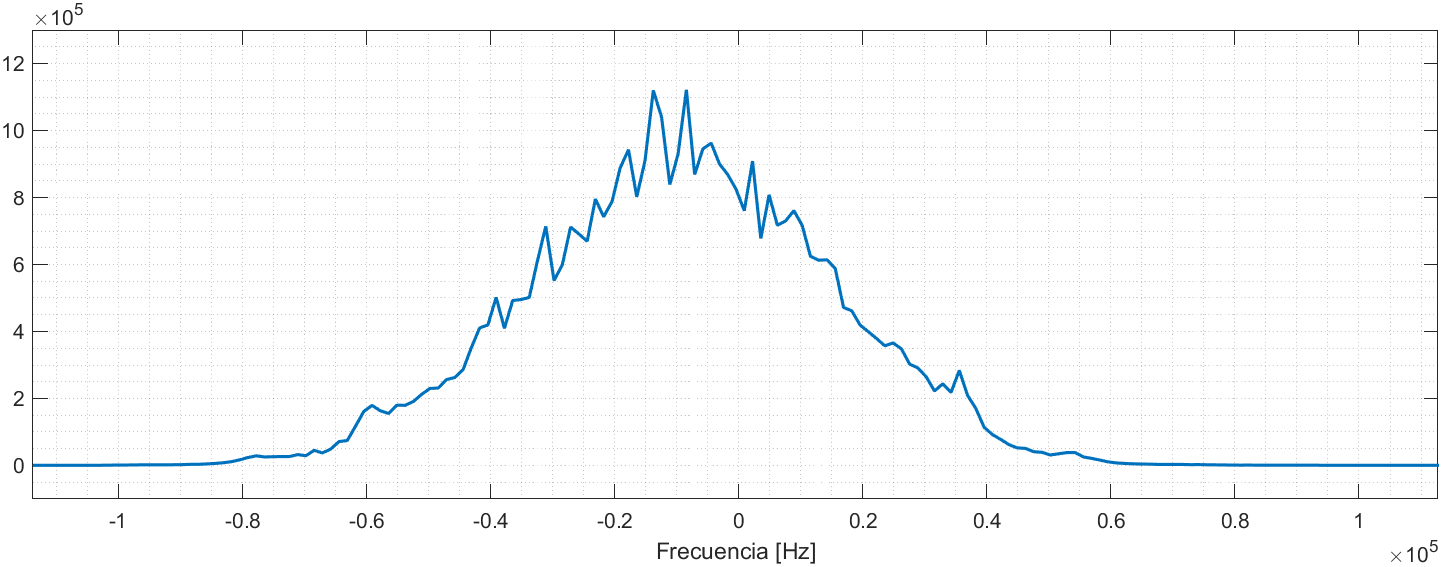
\includegraphics[width=\columnwidth]{images/2.3-diezmando.png}
    \caption{Espectro diezmado con $N_{1}=9$}
    \label{fig:imagen6}
\end{figure}
En este punto, ya se puede intentar obtener el mensaje \textit{MPX} descripto en la \hyperref[fig:imagen2]{Imagen 2}. Como el mensaje esta contenido en la fase de la señal, esto se modela como:
$$
f(t) = f_{c} + \underbrace{\dfrac{1}{2\pi} \dfrac{d\phi}{dt}}_{f_{d}}
$$
Entonces si:
$$
f_{d} = K_{f} \cdot m(t)
\hspace{2mm}\to\hspace{2mm}
m(t) = \dfrac{f_{d}}{2\pi K_{f}} \cdot \dfrac{d\phi}{dt}
$$
Como está definida la máxima desviación sobre la portadora siendo este valor de $75kHz$, se puede pensar que el mensaje entonces ya esta normalizado, dejando entonces $max\{m(t)\}=1$. En base a esto, la constante $K_{f}$ se puede calcular como:
$$
max\{f_{d}\} = K_{f} \cdot max\{m(t)\}
\hspace{2mm}\to\hspace{2mm}
K_{f} = 75kHz
$$
Ya teniendo este valor, solo resta usar la función \texttt{unwrap()} para eliminar los saltos de fase y luego aproximar la derivada con la función \texttt{diff()} junto a la frecuencia de muestreo para así obtener el mensaje MPX.
\begin{figure}[H]
    \centering
    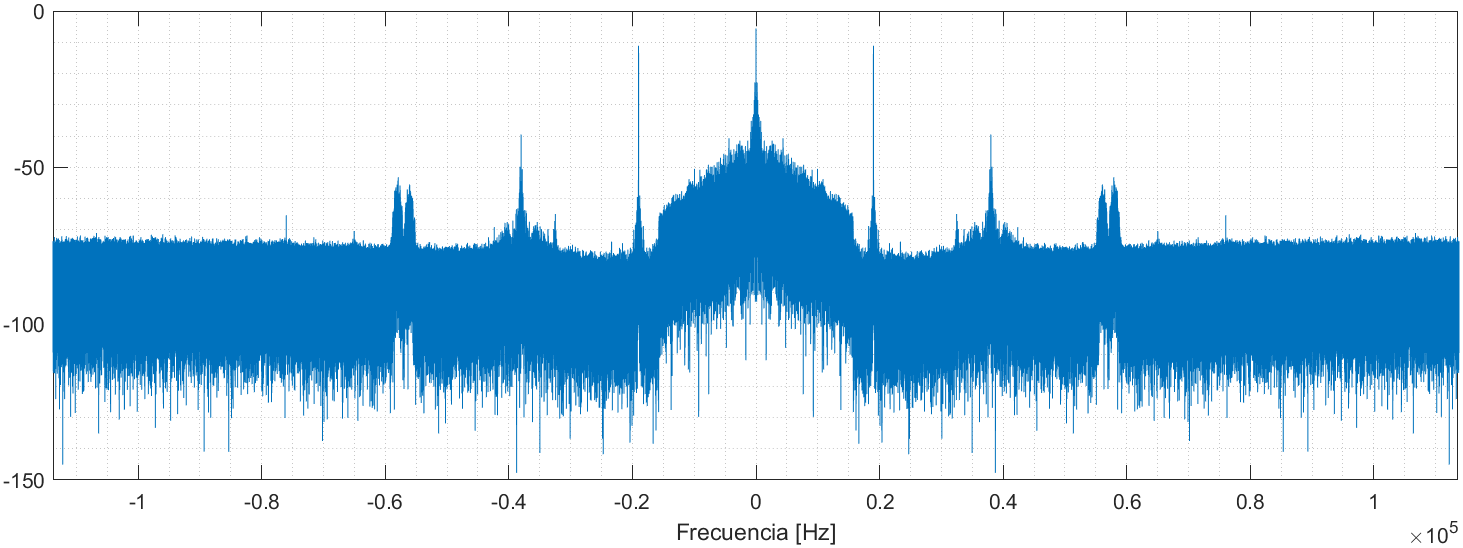
\includegraphics[width=\columnwidth]{images/2.4-mpx-completo.png}
    \caption{Espectro del mensaje MPX}
    \label{fig:imagen7}
\end{figure}
En esta ultima imagen, se puede observar que el mensaje $m(t)$ posee las características de la señal MPX, con una señal piloto de $19kHz$ y la señal de audio de $38kHz$. Finalmente, se ve en menor medida que existe espectro centrado en los $57kHz$ que corresponde a la señal de RDS.

Para obtener de forma sencilla el audio se utilizará unicamente la componente L+R, la cual es el espectro de la señal monoaural. Para esto se realiza un filtrado de la señal MPX en la banda de $0$ a $15kHz$ pero en este caso utilizando un filtro de orden $20$ para lograr mas selectividad ya que dejando el filtro de orden $5$ se requiere colocar la frecuencia de corte por debajo de los $8kHz$ atenuando la señal de audio que se quiere obtener.
\begin{figure}[H]
    \centering
    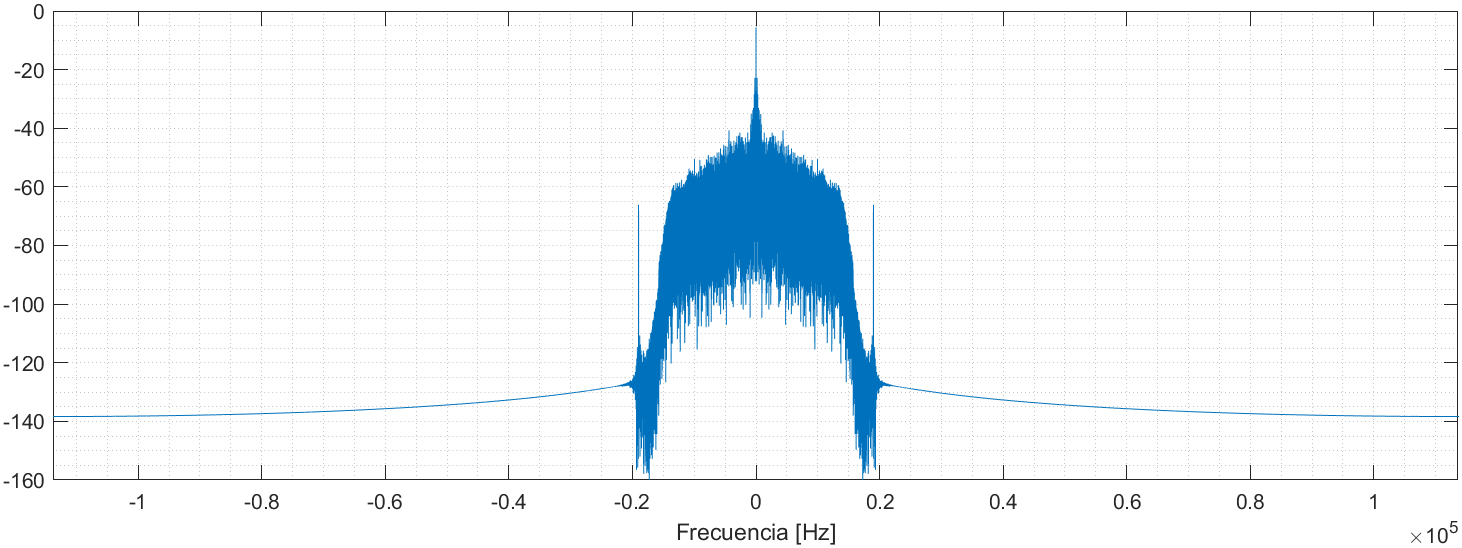
\includegraphics[width=\columnwidth]{images/2.5-mpx-filtrado.png}
    \caption{Espectro del mensaje MPX Filtrado}
    \label{fig:imagen8}
\end{figure}
Finalmente, se realiza un diezmado para lograr que la frecuencia de muestreo sea lo mas cercana a los $48kHz$, ya que en este punto, la $f^{*}_{s}=f_{s}/N_{1}$, entonces si busco los $48kHz$ requiero:
$$
f^{**}_{s} = \frac{f_{s}}{N_{1} N_{2}} = 48kHz
\hspace{2mm}\to\hspace{2mm}
N_{2} \approx 5
$$
Usando esto, la frecuencia de muestreo final sera de $f_{s} \approx 45kHz$ y graficando el espectro se puede ver:
\begin{figure}[H]
    \centering
    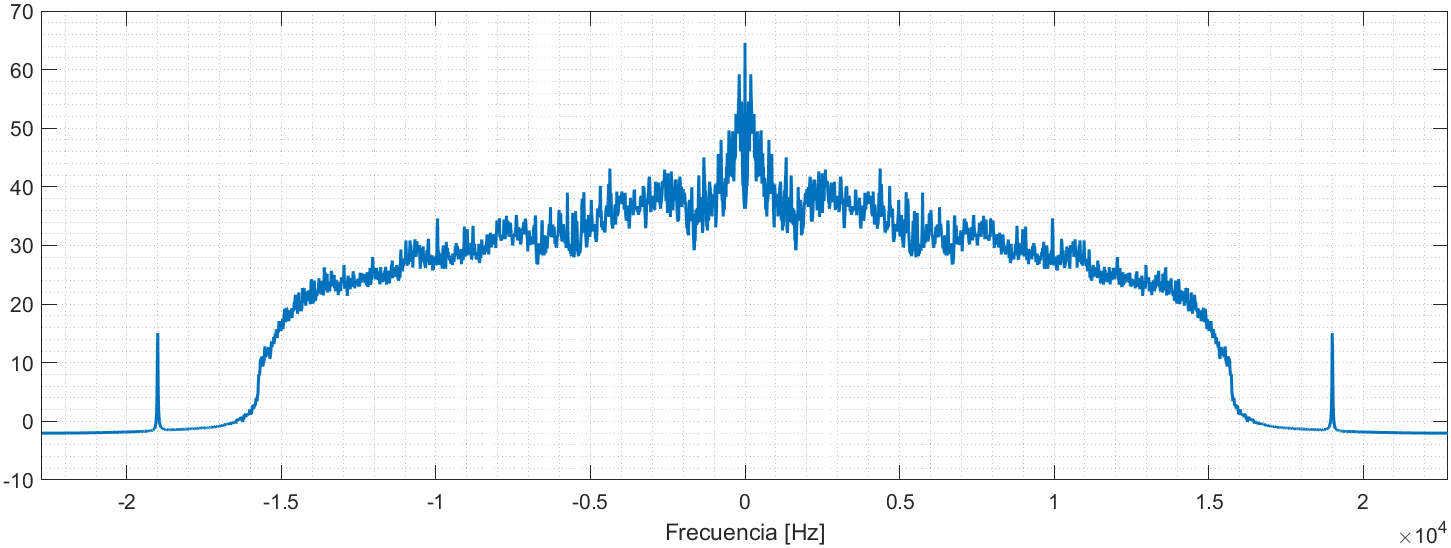
\includegraphics[width=\columnwidth]{images/2.6-mpx-final.png}
    \caption{Espectro audible (L+R)}
    \label{fig:imagen9}
\end{figure}
Finalmente, se puede escuchar el audio de la señal de radio FM en la frecuencia de $103.7 MHz$. Para esto se utilizó la función \texttt{soundsc()} de MatLab, la cual reproduce la señal de audio en tiempo real.

		
		
		\vspace{1cm}
		\hrule
		
		% Bibliografia
		\nocite{*}	% Permite mostrar todo, aunque no este citado
		\printbibliography[title=Bibliografía]
		
	\end{multicols*}
	
	
	
\end{document}